\documentclass{cmn}

\newlength\width
\setlength\width{12mm}
\newlength\height
\setlength\height{9mm}

\begin{document}
  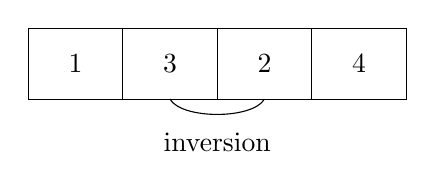
\begin{tikzpicture}
    \begin{scope}
      \draw (0,0) -- ++(4*\width,0) -- ++(0,\height) -- ++(-4*\width,0) -- cycle;
      \foreach \i in {1,...,3} {
        \draw (\i*\width,0) -- ++(0,\height);
      }
      \foreach[count=\i] \n in {1,3,2,4} {
        \node at (-\width/2+\i*\width,\height/2) {\n};
      }

      \draw (3*\width/2,0) .. controls +(-60:3mm) and +(-120:3mm) .. ++(\width,0);

      \node at (2*\width,-5.5mm) {inversion};
    \end{scope}
  \end{tikzpicture}
\end{document}
